\documentclass[journal]{IEEEtran}
\usepackage[a5paper, margin=10mm, onecolumn]{geometry}
\usepackage{tfrupee} % Include tfrupee package

\setlength{\headheight}{1cm} % Set the height of the header box
\setlength{\headsep}{0mm}     % Set the distance between the header box and the top of the text

\usepackage{cite}
\usepackage{amsmath,amssymb,amsfonts,amsthm}
\usepackage{algorithmic}
\usepackage{graphicx}
\usepackage{textcomp}
\usepackage{xcolor}
\usepackage{txfonts}
\usepackage{listings}
\usepackage{enumitem}
\usepackage{mathtools}
\usepackage{gensymb}
\usepackage{comment}
\usepackage[breaklinks=true]{hyperref}
\usepackage{tkz-euclide}
\usepackage{multicol}
\newcommand{\brak}[1]{\left( #1 \right)}

% Marks the beginning of the document
\begin{document}
\bibliographystyle{IEEEtran}
\vspace{3cm}
\title{12.9.5.2}
\author{EE24BTECH11017 - D.Karthik}
{\let\newpage\relax\maketitle}
\renewcommand{\thefigure}{\theenumi}
\renewcommand{\thetable}{\theenumi}

\textbf{Exercise} Verify that the given functions are solutions of the corresponding differential equation:
\begin{align}
    \text{Differential Equation: } y' &= \frac{x + y}{x}
\end{align}

\subsection*{Theoretical Solution}

Rewriting the equation:
\begin{align}
    y' &= 1 + \frac{y}{x}
\end{align}
This is a linear differential equation. Rearranging:
\begin{align}
    \frac{dy}{dx} - \frac{y}{x} &= 1
\end{align}
Here, the equation is in the standard form:
\begin{align}
    \frac{dy}{dx} + P(x)y &= Q(x)
\end{align}
where \( P(x) = -\frac{1}{x} \) and \( Q(x) = 1 \).

The integrating factor (IF) is:
\begin{align}
    IF &= e^{\int P(x) dx} = e^{\int -\frac{1}{x} dx} = e^{-\ln x} = \frac{1}{x}
\end{align}

Multiply through by the integrating factor:
\begin{align}
    \frac{1}{x}\frac{dy}{dx} - \frac{1}{x^2}y &= \frac{1}{x}
\end{align}

The left-hand side becomes the derivative of \( \frac{y}{x} \):
\begin{align}
    \frac{d}{dx}\left(\frac{y}{x}\right) &= \frac{1}{x}
\end{align}

Integrate both sides:
\begin{align}
    \frac{y}{x} &= \ln x + C
\end{align}

Multiply through by \( x \) to find \( y \):
\begin{align}
    y &= x\ln x + Cx
\end{align}
Thus, the general solution is:
\begin{align}
    y = x\ln x + Cx
\end{align}

\subsection*{Numerical Solution}
To numerically verify the solution, we use the Improved Euler's Method as follows:
Definition of derivative,
\begin{align}
    f^\prime(y) &\approx \lim_{h\to0}\frac{f(y+h)-f(y)}{h} \\
    f(y+h) &\approx f(y)+hf^\prime(y) \\
    \implies x_{n+1} &\approx x_{n} + h\frac{dx}{dy}\Big|_{x=x_{n}, y=y_{n}}
\end{align}

Difference equation,
\begin{align}
    y_{n+1} &\approx y_n + h \left( 1+ \frac{y_{n}}{x_{n}}  \right), \quad x_{n+1} = x_n + h.
\end{align}
\begin{figure}[h]
    \centering
    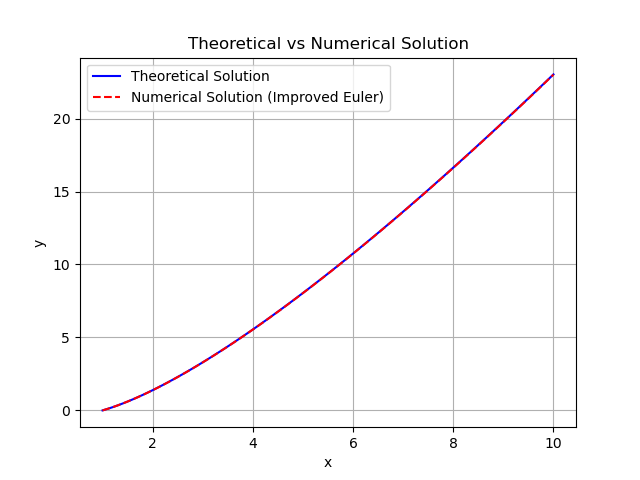
\includegraphics[width=\columnwidth]{figs/Figure_1.png}    
    \end{figure}
\end{document}
